\documentclass[conference]{IEEEtran}
\IEEEoverridecommandlockouts
% The preceding line is only needed to identify funding in the first footnote. If that is unneeded, please comment it out.
\usepackage{cite}
\usepackage{amsmath,amssymb,amsfonts}
\usepackage{algorithmic}
\usepackage{graphicx}
\usepackage{textcomp}
\usepackage{xcolor}
\usepackage{tikz}
\def\BibTeX{{\rm B\kern-.05em{\sc i\kern-.025em b}\kern-.08em
    T\kern-.1667em\lower.7ex\hbox{E}\kern-.125emX}}
\begin{document}

\title{Ceng435 Term Project Part2\\
}

\author{\IEEEauthorblockN{Mert Anıl YILMAZ}
\IEEEauthorblockA{\textit{Group 84} \\
2172211 \\
e2172211@ceng.metu.edu.tr}
\and
\IEEEauthorblockN{Onur Can ÜNAL}
\IEEEauthorblockA{\textit{Group 84} \\
2095966 \\
e2095966@ceng.metu.edu.tr}
}

\maketitle

\section{Abstract}
This project is aimed to send a large file (exactly 5Mb) from a source to a destination by using a UDP-based "Reliable Data Transfer" (RDT) protocol. Checksum approach is used in order to increase reliability. Furthermore, there are routers, r3 for experiment 1, and r1 and r2 for experiment 2. Routers forward packets that are coming from source node. In this project, packets are sent as datagrams by using UDP (User Datagram Protocol) which is a transport layer protocol. Experiment 1 includes pipelining for speeding up and experiment 2 includes both pipelining and multi-homing for speeding up. In addition to that, multi-homing also increases the probability of sending the file to destination even one of routes is down. \\

This report includes design and implementation approach and experiment results.
\section{Problem $\&$ Solution}
Since the file which is aimed to send from source to destination is very large, we cannot send it in a single packet. Therefore, we need to divide it into smaller pieces. \\

At this point, a new problem is encountered which is reliability. In Term Project Part 1, we were responsible to send only one packet each time. The order was not important. However, int Term Project Part 2, in order to obtain the file with the same order, we need to construct a mechanism by using UDP. Since we cannot change transport layer, we have to do our reliability implementations in application layer.
\section{Design $\&$ Implementation Approach}
In Term Project Part 1, we did not need to use pipelining because the aim was to calculate RTT values. However, in this part, pipelining is essential because there are lots of packets to send and without it, the transmission time will increase enormously. \\

Furthermore, we aimed to decrease the transmission time of the file and increase the immunity against link downs by using multi-homing in the second experiment. \\

Furthermore, we added ack and sequence numbers to obtain packets with the right order. Lastly, we used checksum in order to reduce the bit errors. However, checksum approach does not perfectly solve the problems because checksum cannot say there is no bit error. It says that "checksum could not detect any bit error". If a packet fails from checksum test, we ensures that the packet is corrupted but a packet does not fail from checksum test, we cannot ensure that the packet is not corrupted. Actually, there is no checksum test in IPv6. However, our implementation is more close to IPv4 approach since there is checksum test. \\

\subsection{Design $\&$ Implementation for Experiment 1}

\begin{center}
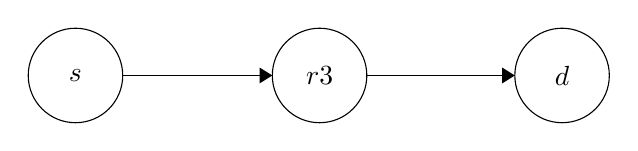
\begin{tikzpicture}[scale=0.2]
\tikzstyle{every node}+=[inner sep=0pt]
\draw [black] (20.9,-19.5) circle (3);
\draw (20.9,-19.5) node {$s$};
\draw [black] (51.8,-19.5) circle (3);
\draw (51.8,-19.5) node {$d$};
\draw [black] (36.4,-19.5) circle (3);
\draw (36.4,-19.5) node {$r3$};
\draw [black] (23.9,-19.5) -- (33.4,-19.5);
\fill [black] (33.4,-19.5) -- (32.6,-19) -- (32.6,-20);
\draw [black] (39.4,-19.5) -- (48.8,-19.5);
\fill [black] (48.8,-19.5) -- (48,-19) -- (48,-20);
\end{tikzpicture}
\end{center}

The file's size is 5000000 bytes. Since each packet can be at most 1000 bytes, and considering ack/sequence number and checksum, we specified that each packet has 800 bytes of the file. It means that we aimed to send from source to destination 6250 different packets(6250*800 = 5000000). Checksum is 32 bytes and ack/sequence number is 4 bytes. The total message size is 32 + 4 + 800 = 836. In our design, each packet includes checksum of the block of ack/sequence number and message content, ack/sequence number and message content, respectively. We decided that not only for message content but also for ack/sequence number, we had to implement checksum check because even message content is not corrupted, if ack/sequence number is corrupted, then the order of the packets will change in destination and the file will be wrong, or since obtaining wrong ack, the new packet that will be sent can be wrong and maybe a packet can be missed to send. \\

We used a hashlib function in order to obtain checksum value (hashlib.md5(message).hexdigest()). This function takes ack/sequence number + message content and converts it into a fixed length sequence which is 32 bytes. However, in hashing, the reverse of the process is not possible. Therefore, we compared checksum value of the packet with the new calculated checksum of received message's sequence number + message content. \\

We only compared these checksums in source and destination. We used r3 for only forwarding since we decided that if we compares checksum in r3, too, the transmission time will increase. In source node, when a response packet arrives, source node implementation controls that whether the ack number received is the same with the sequence number sent. Therefore, checksum is essential for not only destination node but also source node. \\

In order to handle pipelining, we found two solutions which are with threading and without threading. Since we believed that we can handle pipelining with threading much more easier, we decided to implement like this. Our pipelining implementation is similar with Selective Repeat approach but there are some differences. We decided our window size as 8. Therefore, we have 8 threads in source node. These threads are sends packets with a restriction. The restriction is that these threads can only send the packets whose packet numbers are in this window. For example, if window is currently located in the range 0-7, and source threads receive acks of 1,2,3,4,5,6, and 7th packets, since the ack of the packet which has smallest packet no in window is not received yet, the other threads wait. When 0th packet ack is received, window will slide and the smallest packet no will be 8 after that. In the other case that one of source thread receives ack of the smallest packet no in window size, immediately window will slide one unit right. \\

\begin{figure}[htp]
    \centering
    \includegraphics[width=9cm]{pipelining2.png}
    \caption{Source Threads for Experiment 1}
    \label{fig:graph}
\end{figure}

As we can see in Figure 1, we used 8 threads for source implementation. Since we used 8 threads in source implementation, to ensure that each thread sends different packets, we used global variables.

\begin{figure}[htp]
    \centering
    \includegraphics[width=9cm]{pipelining1.png}
    \caption{Global packet no variable to handle pipelining}
    \label{fig:graph}
\end{figure}

For instance, as we can see in Figure 2, packet number is global. Also acked packet information are hold in global. While we were using threads, we needed to be careful since there are common sources (global variables) that are used by each thread. Therefore, we implemented a lock mechanism also by using "with" and it can be seen in Figure 2 also. While we were implementing the first part of the project, we encountered the problem that scripts did not finished, many times. The reason was that some threads did not put back the resources and the other threads waited these resources also. We generally solved the problem by shortening each lock time by using coping the current values of global variables to local. Finally, we used try-except blocks in order to handle timeout issues. When there is a packet loss, since the response packet cannot be received by one of the source threads, then the thread will wait infinitely because of recvfrom() function of the socket. When there is a timeout, it indicates that the packet is lost with high probability, therefore source thread will send the same packet again. After that it waits an ack again. This process will repeat until the right ack value is received by the source thread. This approach can be seen in Figure 3. \\

\begin{figure}[htp]
    \centering
    \includegraphics[width=9cm]{handle_loss.png}
    \caption{Loss handling for source script}
    \label{fig:graph}
\end{figure}

The script in r3 node is very simple. The aim of it, forwarding the packets from source to destination. However, we needed a timeout check in this script because after the router sent the packet to destination, it waited a response packet including ack. This can be seen in Figure 4. If there is a packet loss, then the router cannot obtain the response packet and waits infinitely because of recv() function of the socket. We set the timeout as 0.1 ms as we set timeout in source node. Finally, we used 8 threads in this script, too. Each thread of source script connects with each thread of r3 script. It is like a buffering because the router script can hold 8 packets at the same time without loss.\\

\begin{figure}[htp]
    \centering
    \includegraphics[width=9cm]{router_handle_loss.png}
    \caption{Loss handling for node r3}
    \label{fig:graph}
\end{figure}

The script in destination node is similar with source script but there are some differences also. There are 8 threads in destination script, too. Each thread has one socket binding with a certain port. Each router sends packets one of the destination threads. In destination script, packets are received and then there are some controls. First of all, like source script, destination script has checksum check. If checksums are different, the destination thread generated an ack with value -1. -1 is a special ack which indicates that there is a problem in received packet. This problem can be corruption of packet not only ack corruption but also message content corruption. The destination script sends a response packet including calculated checksum by destination thread, generated ack, and message content. Since we wanted that source thread can use its own calculated checksum, in the destination script, checksum is generated by combination of generated ack and message content. Our generated ack value is the same with the sequence number of the packet if there is no problem (if ack value is not equal to -1). \\

In the destination script, there is also timeout check but it is used for a different purpose. If for a long time, a destination thread cannot receive a packet, then in except block, there is a check whether the smallest received packet no is equal to 6250. If it is so, it means that all packets are received and the threads of destination script must be terminated. \\

In addition to it, we encountered a problem while writing message content inside to output.txt. The main process creates output.txt at the end of the process but since there is no packet received, output.txt file was empty. We solved the problem keeping the main process busy until the end of the communication process.

\subsection{Design $\&$ Implementation for Experiment 2 (Multi-homing)}

\begin{center}
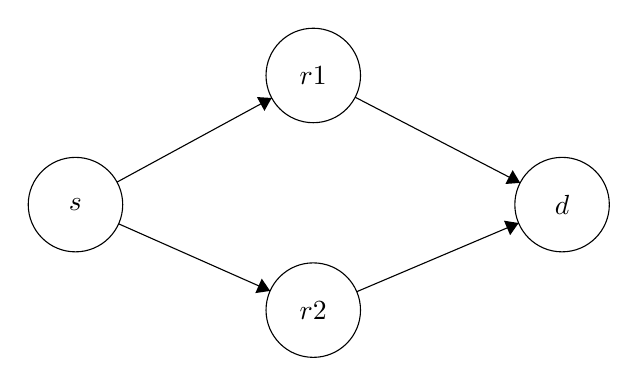
\begin{tikzpicture}[scale=0.2]
\tikzstyle{every node}+=[inner sep=0pt]
\draw [black] (20.9,-19.5) circle (3);
\draw (20.9,-19.5) node {$s$};
\draw [black] (51.8,-19.5) circle (3);
\draw (51.8,-19.5) node {$d$};
\draw [black] (36,-11.3) circle (3);
\draw (36,-11.3) node {$r1$};
\draw [black] (36,-26.2) circle (3);
\draw (36,-26.2) node {$r2$};
\draw [black] (23.54,-18.07) -- (33.36,-12.73);
\fill [black] (33.36,-12.73) -- (32.42,-12.67) -- (32.9,-13.55);
\draw [black] (38.66,-12.68) -- (49.14,-18.12);
\fill [black] (49.14,-18.12) -- (48.66,-17.31) -- (48.2,-18.19);
\draw [black] (23.64,-20.72) -- (33.26,-24.98);
\fill [black] (33.26,-24.98) -- (32.73,-24.2) -- (32.32,-25.12);
\draw [black] (38.76,-25.03) -- (49.04,-20.67);
\fill [black] (49.04,-20.67) -- (48.11,-20.52) -- (48.5,-21.44);
\end{tikzpicture}
\end{center}

The second experiment have similarities with the first one but there are some differences. Firstly, we had to use two routers, r1 and r2, not one router like the first experiment. Secondly, we need to implement multi-homing and we had to consider link downs. \\

In order to obtain a generic code for both first and second experiment, we tried to design an appropriate solution. Our first thought was a design that source script had 16 threads, each router script had 8 threads and destination script had 16 threads also. There was a global value hold the packet number that is not sent yet. Each 16 threads used this number in order to indicate which packet will send. After we implemented this, we noticed that there was a problem that since packet number is a global and all 16 threads used it, they waited each other. The windows size was common for these two routes and it was problematic. We needed to two different global packet number in order to avoid this type of waiting. However, we could not handle it. Therefore, we focused on another solutions. \\

The second solution we thought was that dividing packets into two group and each group was sent one of two routes. We used two global packet number, and their initial values are 0 and 3125, respectively. It means that the first half of the packets would be sent by the first route, s-r1-d, and the other half would be sent by the other route, s-r2-d. We implemented this solution and we obtained the same file in destination node. However, since we did not consider link down issue, our implementation was not worked for this case. We tried to handle it but we needed to significant changes in our first script implementations. Therefore, we abandoned this solution also. \\

The last solution we thought was very simple. Since we had only two router, we decided to send packets with two ways, the beginning of the file and the end of the file. To be clear, s-r1-d route's threads send packets starting with packet number as 0 and s-r2-d route's threads send packets starting with packet number 6249 which is the last packet. \\

In order to implement this approach, we needed two different packet number in global. There are 16 source threads, 8 router threads for each and 16 destination threads. This approach enabled us not to change our first experiment solution much. Actually, for the route 1 (s-r1-d), the implementation is quite similar. There are only small changes such as termination controls. For instance, in experiment 1, source threads are terminated when exceeding the last packet while in experiment 2, source threads are terminated when smallest unacked value for route 1 is bigger than biggest unacked value for route 2. It means that all packets are sent. \\

For instance, 8 threads will execute destination1 function and the other 8 threads will execute destination2 function. These functions are very similar but as we stated earlier, one of them received packets starting from beginning of the file and the other received packets starting from the end of file. Our destination threads can be seen in Figure 5. \\

\begin{figure}[htp]
    \centering
    \includegraphics[width=9cm]{multihoming2.png}
    \caption{Threads for multi-homing}
    \label{fig:graph}
\end{figure}


In order to handle link down cases, we thought that if we set a timeout value large enough, and if one of threads has 100 times timeout successively, it means that the link of the route is down. It was a hypothetical approach but we did some calculations about it: \\

for 5$\%$ packet loss:\\
the probability that the reason of timeout is not due to packet loss: 95$\%$ \\
if there are 100 times timeout successively, then the probability that the successive timeouts are not due to packet loss: \\
(95$\%$) $^{100}$ = 0.00592052922 \\

Since the probability is very small, we thought to use a timeout counter in order to indicate the link down and then, we thought to terminate the threads. However, we noticed that even a link is down, source threads can try to send the packets and this is not a problem for our design. Since smallest unacked value and biggest unacked value are in global, source threads of the route which is down are terminated also when smallest unacked value for route 1 is bigger than biggest unacked value for route 2. The other parts such as checksum calculations, re-transmission of packets, ack handling are parallel with the implementation of experiment 1. When a source thread does not receive an ack by exceeding the threshold time, the packet is re-sended again. Similarly, if router threads does not receive a response from destination thread, then the router thread re-sends the packet received from the source. Since the design for both experiment are similar, we did not need to change the first implement significantly. \\

In experiment 1, we ended a thread when exceeding the last packet no. For the second experiment, we used another control mechanism. For instance, in destination script, when r1-rcvbase exceeds r2-rcvbase, then the thread is terminating. This can be seen in Figure 6. \\

\begin{figure}[htp]
    \centering
    \includegraphics[width=9cm]{multihoming1.png}
    \caption{Terminating control mechanism for multi-homing}
    \label{fig:graph}
\end{figure}

All routers have the same scripts except for IP and port numbers. We run the source script with parameter "1" or "2". "1" indicates that this is for experiment 1 and experiment 1 block will be executed. Similarly, "2" indicates that this is for experiment 2 and experiment 2 block will be executed. \\

\section{Link Down}
In our implementation, when a link is down, the rest of the packets will be transmitted from the other link. After we completed all implementation process, we tried our code whether it handles the issue or not. We tried it with packet loss 15$\%$ by using command, ip link set dev <interface> down. In figure 7, we can see that when transmission process is run, we typed the command for s-r1. This figure shows that when we typed the command, after we looked at the connections wih ip a command, we see that link is down.

\begin{figure}[htp]
    \centering
    \includegraphics[width=9cm]{link_down.png}
    \caption{Link down command usage}
    \label{fig:graph}
\end{figure}

\section{Methodology}
We used Python as programming language in Term Project Part 2, too. We used the same libraries with Part 1 and additional library, hashlib in order to implement checksum approach in our solution. We used UDP for transport layer but we implemented our RDT in order to create reliable communication between source and destination. We used time library in order to do experiments.
\section{Motivation}
This part of the project includes extensive multi-threading knowledge because of our implementation choice. At the end of the project, we did not adequate to manage all threads with global common resources but we encountered lots of errors and we increased our knowledge about the topic. Furthermore, we learned how we obtain a reliable communication even we are using UDP. Our instructor explained that in a lecture but this project enables us to experience it at first hand.
\section{Experiments}
We conducted 2 experiments in this part of the term project. The first experiment is observing the results that we obtained by sending file over the shortest path, s - r3 - d. For the second experiment, we sent file by using multi-homing implementation, using s - r1 - d and s - r2 - d paths simultaneously. \\

For the calculation of the file transmission time, since there is no specification that was given to us about how we could calculate, we printed out the time that the file transmission started from the source node on the terminal of source node, and we printed out the time that the file transmission ended from the destination node on the terminal of destination node. The nodes were not synchronized, and so their time-zones were different. We may get the unexpected results because of that. To make them synchronized, we used the command "sudo ntpdate -u pool.ntp.org" in the terminals of the nodes after connecting to them. We typed it before running the Python scripts. After the scripts were terminated, we subtracted the start time of the file transmission from the end time of the file transmission, and we got the results in seconds. \\

For the plot of the experiment, we needed to find margin of errors. To find them, we used the following formula: \\

$e = z * \dfrac{\sigma}{\sqrt{n}}$ \\

Here, $e$ is the margin of error, $\sigma$ is the standard deviation of end-to-end delays, and $n$ is the number of packets that had been sent. Since we use 95\% confidence interval, $z$ value is $1.96$. We plotted the graph with respect to those values by using GNU Octave. \\

\subsection{Experiment 1}
For the first experiment, we sent 5MB file from source node to destination node through router 3, r3 node. We conducted the experiment according to 3 different cases. Firstly, we configured all links from each of s, r3, and d nodes with the packet loss of 5 percentage and the delay of 3ms. Then, secondly, we configured all links from each of s, r3, and d nodes with the packet loss of 15 percentage and the delay of 3ms. And finally, for the third case, we configure all links from each of s, r3, and d nodes with the packet loss of 38 percentage and the delay of 3ms. For the configurations, we used the configuration files that had been given to us for the first part of the term project, and we wrote our configuration scripts. To write those scripts, we used netem/tc commands that we wrote in README file. \\

We run our scripts on node s, r3, and d for each 3 cases (5, 15, and 38 percentage of packet loss), respectively. We run the scripts until we got a result such that the margin of error is less than 2.5\%. \\

For 5\% packet loss case, we run our scripts 8 times. We got 93.79 seconds as the mean value, 2.9665468 as the standard deviation, and 2.056 as the margin of error. The percentage of the margin of error is 2.19 \%, which is less than 2.5 \%. For 15\% packet loss case, we run our scripts 5 times. We got 345.474 seconds as the mean value, 8.99793 as the standard deviation, and 7.887 as the margin of error. The percentage of the margin of error is 2.28 \%, which is less than 2.5 \%. For 38\% packet loss case, we run our scripts 4 times. We got 2238.1525 seconds as the mean value, 51.943 as the standard deviation, and 50.904 as the margin of error. The percentage of the margin of error is 2.27 \%, which is less than 2.5 \%. The graph that we plotted with respect to those values can be seen from Figure 8. \\

By looking at figure, we observed that file transmission time increases when the packet loss percentage increases. It is meaningful since whenever there is a packet loss, the source re-transmits that packet, and so there will be some delay. If the probability of packet loss is higher, then, the file transmission time will be later than expected.

\begin{figure}[htp]
    \centering
    \includegraphics[width=9cm]{graph_exp1.png}
    \caption{Packet Loss vs File Transfer Time}
    \label{fig:graph}
\end{figure} 

\subsection{Experiment 2}

For the second experiment, we sent 5MB file from source node to destination node through both router 1, r1, and router 2, r2, simultaneously (multi-homing). We conducted the experiment according to 3 different cases. Firstly, we configured all links from each of s, r1, r2, and d nodes with the packet loss of 5 percentage and the delay of 3ms. Then, secondly, we configured all links from each of s, r1, r2, and d nodes with the packet loss of 15 percentage and the delay of 3ms. And finally, for the third case, we configure all links from each of s, r1, r2, and d nodes with the packet loss of 38 percentage and the delay of 3ms. For the configurations, we used the configuration files that had been given to us for the first part of the term project, and we wrote our configuration scripts. To write those scripts, we used netem/tc commands that we wrote in README file. \\

We run our scripts on node s, r1, r2, and d for each 3 cases (5, 15, and 38 percentage of packet loss), respectively. We run the scripts until we got a result such that the margin of error is less than 2.5\%. To calculate file transmission time, we did not drop any link to get lower file transmission time. \\

For 5\% packet loss case, we run our scripts 5 times. We got 49.226 seconds as the mean value, 1.39695 as the standard deviation, and 1.224 as the margin of error. The percentage of the margin of error is 2.49 \%, which is less than 2.5 \%. For 15\% packet loss case, we run our scripts 5 times. We got 162.76 seconds as the mean value, 4.238832 as the standard deviation, and 3.716 as the margin of error. The percentage of the margin of error is 2.28 \%, which is less than 2.5 \%. For 38\% packet loss case, we run our scripts 5 times. We got 690.19 seconds as the mean value, 18.5186 as the standard deviation, and 16.232 as the margin of error. The percentage of the margin of error is 2.35 \%, which is less than 2.5 \%. The graph that we plotted with respect to those values can be seen from Figure 9. \\

\begin{figure}[htp]
    \centering
    \includegraphics[width=9cm]{exp2.png}
    \caption{Packet Loss vs File Transfer Time}
    \label{fig:graph}
\end{figure} 

By looking at figure, we observed that file transmission time increases when the packet loss percentage increases. It is meaningful since whenever there is a packet loss, the source re-transmits that packet, and so there will be some delay. If the probability of packet loss is higher, then, the file transmission time will be later than expected. \\

Moreover, we observed that file transmission time of experiment 1 took nearly 2 times higher than file transmission time of experiment 2. This makes sense because we used multi-homing approach in experiment 2. We divided the file into 2, and we sent the first part through s - r1 - d, and the second part through s - r2 - d. Thus, file transmission time is reduced by half in experiment 2. It means that multi-homing approach reduces transmission time significantly. Each two router in experiment 2 has buffer size as 8 and it means that the capacity of the buffer doubles. In addition to it, since we use two different link in multi-homing, we can transmit packets with reduced queuing delay. \\

\section{Workload}
We are designed our solutions together and we shared the scripts after that. For instance one of us wrote the source script for the second experiment while the other wrote the destination script for the second experiment. We had lots of errors and we generally swapped the scripts in order to find the problem. We did together experiment parts together. One of us calculated and drew graphs and the other wrote the results in experiment part of the report. The rest of the report were written together. The workload of each member the team is fair.

\section{Reference}
Kurose, J. F., \& Ross, K. W. (2017). Computer networking: a top-down approach. Pearson.


\end{document}
